%
% rodrigues.tex
%
% (c) 2022 Prof Dr Andreas Müller, OST Ostschweizer Fachhochschule
%
\section{Rodrigues-Formeln
\label{buch:orthogonalitaet:section:rodrigues}}
\rhead{Rodrigues-Formeln}
Die Drei-Term-Rekursionsformel ermöglicht Werte orthogonaler Polynome
effizient zu berechnen.
Die Rekursionsformel erhöht den Grad eines Polynoms, indem mit $x$ 
multipliziert wird.
mit der Ableitung kann man den Grad aber auch senken, man könnte daher
auch nach einer Rekursionsformel fragen, die bei einem Polynom hohen
Grades beginnt und mit Hilfe von Ableitungen zu geringeren Graden
absteigt.
Solche Formeln heissen {\em Rodrigues-Formeln} nach dem Entdecker Olinde
\index{Rodriguez, Olinde}%
Rodrigues, der eine solche Formal als erster für Legendre-Polynome
gefunden hat.

In diesem Abschnitt sei $p_n(x)$ eine bezüglich des Skalarproduktes
$\langle\,\;,\;\rangle_w$ auf dem Intervall $[a,b]$ orthogonale Familie
von Polynomen mit genaum dem Grad $\deg p_n=n$.
Die Skalarprodukte sollen 
\[
\langle p_n,p_m\rangle_w = h_n\delta_{nm}
\]
sein.

%
% Pearsonsche Differentialgleichung
%
\subsection{Pearsonsche Differentialgleichung}
Die {\em Pearsonsche Differentialgleichung} ist die Differentialgleichung
\begin{equation}
B(x) y' - A(x) y = 0,
\label{buch:orthogonal:eqn:pearson}
\end{equation}
\index{Differentialgleichung!Pearsonsche}%
\index{Pearsonsche Differentialgleichung}%
wobei $B(x)$ ein Polynom vom Grad höchstens $2$ ist und $A(x)$ ein
höchstens lineares Polynom.
Die Gleichung~\eqref{buch:orthogonal:eqn:pearson}
kann gelöst werden, wenn $y$ und $B(x)$ keine Nullstellen  haben.
Dann kann man die Gleichung umstellen in
\[
\frac{y'}{y}
=
(\log y)'
=
\frac{A(x)}{B(x)}
\qquad\Rightarrow\qquad
y
=
\exp\biggl(
\int\frac{A(x)}{B(x)}
\,dx
\biggr)
.
\]
Im Folgenden nehmen wir zusätzlich an, dass an den Intervallenden
\begin{equation}
\lim_{x\to a+} w(x)B(x) = 0,
\qquad\text{und}\qquad
\lim_{x\to b-} w(x)B(x) = 0
\end{equation}
gilt.

Falls $w(x)$ an den Intervallenden einen von $0$ verschiedenen
Grenzwert hat, bedeutet dies, dass $B(a)=B(b)=0$ sein muss.
Falls $w(x)$ am Intervallende divergiert, muss $B(x)$ dort eine
Nullstelle höherer Ordnung haben, was aber für ein Polynom
zweiten Grades nicht möglich ist.

%
% Rekursionsformel
%
\subsection{Rekursionsformel}
Multiplikation mit $B(x)$ wird den Grad eines Polynomes typischerweise 
um $2$ erhöhen, die Ableitung wird ihn wieder um $1$ reduzieren.
Etwas formeller kann man dies wie folgt formulieren:

\begin{satz}
\index{Satz!Rodrigues-Rekursionsformel}%
Für alle $n\ge 0$ ist
\begin{equation}
q_n(x)
=
\frac{1}{w(x)}
\frac{d^n}{dx^n} B(x)^n w(x)
\label{buch:orthogonalitaet:rodrigues:eqn:rekursion}
\end{equation}
ein Polynom vom Grad höchstens $n$.
\end{satz}

\begin{proof}[Beweis]
Wenn $r_0(x)$ irgend eine differenzierbare Funktion ist, dann ist
\begin{align*}
\frac{d^n}{dx^n}
r_0(x) B(x)^n w(x)
&=
\frac{d^{n-1}}{dx^{n-1}}\frac{d}{dx} r_0(x) B(x)^n w(x)
\\
&=
\frac{d^{n-1}}{dx^{n-1}}
\bigl(r_0'(x)B(x)+ nr_0(x)B'(x)B(x)^{n-1}w(x) + r_0(x)B(x)^n w'(x) \bigr)
\\
&=
\frac{d^{n-1}}{dx^{n-1}}
(\underbrace{r_0'(x)B(x)+nr_0(x)B'(x)+r_0(x)A(x)}_{\displaystyle = r_1(x)})
B(x)^{n-1} w(x)
\\
&=
\frac{d^{n-1}}{dx^{n-1}} r_1(x)B^{n-1}(x) w(x).
\end{align*}
Iterativ lässt sich eine Folge von
Funktionen $r_k(x)$ definieren, für die Rekursionsformel
\begin{equation}
r_k(x) = r_{k-1}'(x)B(x) + \bigl((n+1-k)B'(x) + A(x)\bigr)r_{k-1}(x)
\label{buch:orthogonal:rodrigues:rekursion:beweis1}
\end{equation}
gilt.
Wenn $r_0(x)$ ein Polynom ist, dann sind alle Funktionen $r_k(x)$
ebenfalls Polynome.
Aus der Konstruktion kann man schliessen, dass
\[
\frac{d^n}{dx^n} r_0(x) B(x)^n w(x)
=
r_n(x) w(x).
\]
Insbesondere folgt für $r_0(x)=1$, dass die $n$-te Ableitung den
Faktor $w(x)$ enthält und dass somit $r_n(x)=q_n(x)$ ein Polynom ist.

Wir müssen auch noch den Grad von $r_k(x)$ bestimmen, wobei wir
wieder von $r_0(x)=1$ ausgehen.
Wir behaupten, dass $\deg r_k(x)\le k$ ist, und beweisen dies
mit vollständiger Induktion.
Für $k=0$ ist $\deg r_0(x) = 0 \le k$ die Induktionsverankerung.

Wir nehmen jetzt also an, dass $\deg r_{k-1}(x)\le k-1$ ist und
verwenden 
\eqref{buch:orthogonal:rodrigues:rekursion:beweis1} um den Grad zu berechnen:
\begin{equation*}
\deg r_k(x)
=
\max \bigl(
\underbrace{\deg(r_{k-1}'(x) B(x))}_{\displaystyle (k-1) -1 + 2}
,
\underbrace{\deg(r_{k-1}(x)B'(x))}_{\displaystyle \le (k-1)+1}
,
\underbrace{\deg(r_{k-1}(x)A(x))}_{\displaystyle \le (k-1)+1}
\bigr)
\le k.
\end{equation*}
Damit ist der Induktionsschritt und $\deg r_k(x)\le k$ bewiesen.
Damit ist auch gezeigt, dass $\deg q_n(x)\le n$.
\end{proof}

Die Rodrigues-Formel~\eqref{buch:orthogonalitaet:rodrigues:eqn:rekursion}
produziert eine Folge von Polynomen aufsteigenden Grades, es ist aber
noch nicht klar, dass diese Polynome bezüglich des gewählten Skalarproduktes
orthogonal sind.
Dies ist der Inhalt des folgenden Satzes.

\begin{satz}
\index{Satz!Rodrigues-Formel für orthonormierte Polynome}%
Es gibt Konstanten $c_n$ derart, dass
\[
p_n(x)
=
\frac{c_n}{w(x)} \frac{d^n}{dx^n} \bigl(B(x)^n w(x)\bigr) 
\]
gilt.
\end{satz}

\begin{proof}[Beweis]
Wir zeigen, dass die Polynome orthogonal sind auf allen Monomen
von geringerem Grad.
\begin{align*}
\langle q_n, x^k\rangle_w
&=
\int_a^b q_n(x)x^kw(x)\,dx
\\
&=
\int_a^b \frac{1}{w(x)}
\biggl(\frac{d^n}{dx^n}\bigl(B(x)^n w(x)\bigr)\biggr)
x^k w(x)\,dx
\\
&=
\int_a^b \frac{d^n}{dx^n}\bigl(B(x)^n w(x)\bigr) x^k \,dx
\\
&=
\biggl[\frac{d^{n-1}}{dx^{n-1}}\bigl(B(x)^n w(x)\bigr) x^k \biggr]_a^b
-
\int_a^b \frac{d^{n-1}}{dx^{n-1}}\bigl(B(x)^n w(x)\bigr)kx^{k-1}\,dx
\end{align*}
Durch $n$-fache Iteration wird das Integral auf $0$ reduziert.
Es bleiben nur die eckigen Klammern stehen, doch wenn man die Produktregel
auswertet, bleibt immer mindestens ein Produkt $B(x)w(x)$ stehen,
nach den Voraussetzungen an den Grenzwert dieses Produktes an den
Intervallenden verschwinden diese Terme alle.
Damit sind die $q_n(x)$ Polynome, die $w$-orthogonal sind auf allen
$x^k$ mit $k<n$.

Die Polynome $q_k(x)$ mit $k< n$ haben Grad $<n$ und sind daher
Linearkombinationen von Monomen vom Grad $<n$.
Soeben wurde gezeigt, dass $q_n(x)$ orthogonal auf diesen Monomen
ist, also auch auf $q_k(x)$ mit $k<n$.
Damit ist gezeigt, dass Polynome $q_n(x)$ eine orthogonale Familie
von Polynomen bilden.
Durch Normierung müssen sich daraus die Polynome $p_n(x)$ ergeben.
\end{proof}

\subsection{Differentialgleichung}
Man kann auch zeigen (siehe z.~B.~\cite{buch:pearsondgl},
dass die orthogonalen Polynome, die die
Rodrigues-Formel liefert, einer Differentialgleichung zweiter 
Ordnung genügen, deren möglicherweise nicht konstante Koeffizienten
sich direkt aus $A(x)$, $B(x)$ und $w(x)$ bestimmen lassen.

\subsection{Beispiel}
Im folgenden zeigen wir, wie sich für viele der früher eingeführten
Gewichtsfunktionen Rodrigues-Formeln für die zugehörigen orthogonalen
Polynome konstruieren lassen.

%
% Legendre-Polynome
%
\subsubsection{Legendre-Polynome}
Legendre-Polynome sind orthogonale Polynome zum Standardskalarprodukt
mit $w(x)=1$.
Die Pearsonsche Differentialgleichung ist für $A(x)=0$ immer erfüllt.
Die Randbedingung bedeutet wegen $w(x)=1$, dass $B(x)$ an den
Endpunkten des Intervalls verschwinden muss.
Da $B(x)$ ein Polynom höchstens vom Grad $2$ ist, muss $B(x)$ ein
Vielfaches von $(x-1)(x+1)=x^2-1$ sein.
Die Rodrigues-Formel für die Legendre-Polynome hat daher die Form
\[
P_n(x)
=
c_n
\frac{d^n}{dx^n}
(x^2-1)^n,
\]
darin müssen die Konstanten $c_n$ noch bestimmt werden.
In der für die Legendre-Polynome gewählten Normierung ist
\[
c_n = \frac1{2^n n!}
\qquad\text{und damit}\qquad
P_n(x)
=
\frac{1}{2^nn!}
\frac{d^n}{dx^n}
(x^2-1)^n.
\]

%
% Hermite-Polynome
%
\subsubsection{Hermite-Polynome}
Die Hermite-Polynome sind auf ganz $\mathbb{R}$ definiert und verwenden
die Gewichtsfunktion
\[
w(x) = e^{-x^2}.
\]
Für jedes beliebige Polynome $B(x)$, auch für höheren Grad als $2$, ist
\[
\lim_{x\to-\infty} B(x) w(x)
=
\lim_{x\to-\infty} B(x)e^{-x^2}
=
0
\qquad\text{und}\qquad
\lim_{x\to\infty} B(x) w(x)
=
\lim_{x\to\infty} B(x)e^{-x^2}
=
0,
\]
die Randbedingung der Pearsonschen Differentialgleichung ist also
immer erfüllt.

Die Ableitung der Gewichtsfunktion ist
\[
w'(x) = -2xe^{-x^2}.
\]
Eingesetzt in die Pearsonsche Differentialgleichung findet man
\[
\frac{w'(x)}{w(x)}
=
\frac{-2xe^{-x^2}}{e^{-x^2}}
=
\frac{-2x}{1}
\]
und daher
\[
A(x) = -2x
\qquad\text{und}\qquad
B(x) = 1.
\]
Die Gradbedingung ist also immer erfüllt und es folgt die Rodrigues-Formel
für die Hermite-Polynome
\index{Hermite-Polynom}%
\index{Polynome!Hermite}%
\begin{equation}
H_n(x)
=
c_n
e^{x^2}\frac{d^n}{dx^n} e^{-x^2}
=
(-1)^n
e^{x^2}\frac{d^n}{dx^n} e^{-x^2}.
\label{buch:orthogonal:eqn:hermite-rodrigues}
\end{equation}

Die Hermite-Polynome können mit der Rodrigues-Formel berechnet werden,
aber die Form~\eqref{buch:orthogonal:eqn:hermite-rodrigues} ist dazu
nicht gut geeignet.
Zur Vereinfachung dient die Berechnung 
\[
-\frac{d}{dx}
\bigl(
e^{-x^2}f(x)
\bigr)
=
2xe^{-x^2}f(x)
-
e^{-x^2}f'(x)
=
e^{-x^2}
\biggl(-\frac{d}{dx}+2x\biggr)
f(x),
\]
nach der der Ableitungsoperator mit dem Faktor $e^{-x^2}$ 
vertauscht werden kann, wenn er durch die grosse Klammer auf der
rechten Seite ersetzt wird.
Die Rodrigues-Formel bekommt daher die Form
\[
H_n(x) = \biggl(2x-\frac{d}{dx}\biggr)^n \cdot 1.
\]

%TODO: Relation zu hypergeometrischen Funktionen $\mathstrut_1F_1$

%\url{https://en.wikipedia.org/wiki/Rodrigues%27_formula}

%
% Jacobi-Gewichtsfunktion
%
\subsubsection{Jacobi-Gewichtsfunktion}
%(%i1) w: (1-x)^a*(1+x)^b;
%                                      a        b
%(%o1)                          (1 - x)  (x + 1)
%(%i2) diff(w,x)/w;
%                        a        b - 1            a - 1        b
%               b (1 - x)  (x + 1)      - a (1 - x)      (x + 1)
%(%o2)          -------------------------------------------------
%                                      a        b
%                               (1 - x)  (x + 1)
%(%i3) q: diff(w,x)/w;
%                        a        b - 1            a - 1        b
%               b (1 - x)  (x + 1)      - a (1 - x)      (x + 1)
%(%o3)          -------------------------------------------------
%                                      a        b
%                               (1 - x)  (x + 1)
%(%i4) ratsimp(q);
%                               (b + a) x - b + a
%(%o4)                          -----------------
%                                     2
%                                    x  - 1
%
Die Jacobi-Gewichtsfunktion 
\index{Jacobi-Gewichtsfunktion}%
\index{Gewichtsfunktion!Jacobi}%
\[
w(x)
=
w^{(\alpha,\beta)}(x)
=
(1-x)^\alpha(1+x)^\beta
\]
hat die Ableitung
\[
w'(x)
=
\beta(1-x)^\alpha(1+x)^{\beta-1}-\alpha(1-x)^{\alpha-1}(1+x)^\beta
\]
und für die linke Seite der Pearsonschen Differentialgleichung findet man
\[
\frac{w'(x)}{w(x)}
=
\frac{
\beta(1-x)^\alpha(1+x)^{\beta-1}-\alpha(1-x)^{\alpha-1}(1+x)^\beta
}{
(1-x)^\alpha(1+x)^\beta
}
=
\frac{\beta-\alpha-(\alpha+\beta)x}{1-x^2}
=
\frac{A(x)}{B(x)}.
\]
Die Polynome
\[
A(x) = \beta-\alpha-(\alpha+\beta)x
\qquad\text{und}\qquad
B(x) = 1-x^2
\]
erfüllen die Gradvoraussetzungen für eine Lösung der Pearsonschen
Differentialgleichung, die Anlass zu einer Rodrigues-Formel gibt.
Die Randbedingungen sind noch zu prüfen: $B(x)$ hat eine Nullstelle
erster Ordnung bei $\pm1$, also ist
\[
\lim_{x\to \pm1\mp} B(x)w(x) = 0
\]
genau dann, wenn $\alpha>-1$ und $\beta>-1$ gilt.
Für $\alpha>-1$ und $\beta>-1$ gibt es daher auch für die Jacobi-Polynome
eine Rodriguez-Formel der Art
\[
P^{(\alpha,\beta)}_n(x)
=
\frac{c_n}{w^{(\alpha,\beta)}(x)}
\frac{d^n}{dx^n}
\bigl((1-x^2)^{n} w^{(\alpha,\beta)}(x)\bigr).
\]
Die Konstanten $c_n$ werden durch die Normierung
% XXX in welchem Abschnitt
festgelegt.

%
% Tschebyscheff-Gewichtsfunktion
%
\subsubsection{Die Tschebyscheff-Gewichtsfunktion}
Die Tschebyscheff-Gewichtsfunktion ist der Spezialfall $a=b=-\frac12$
der Jacobi-Gewichtsfunktion.
\index{Tschebyscheff-Gewichtsfunktion}%
\index{Gewichtsfunktion!Tschebyscheff}%
Die Rodrigues-Formel für die Tschebyscheff-Polynome lautet daher
\[
T_n(x)
=
c_n\sqrt{1-x^2} \frac{d^n}{dx^n}
\frac{(1-x^2)^n}{\sqrt{1-x^2}}
=
\frac{1}{2^nn!} \sqrt{1-x^2}
\frac{d^n}{dx^n} 
\frac{(1-x^2)^n}{\sqrt{1-x^2}},
\]
wobei wir den korrekten Wert von $c_n$ nicht nachgewiesen haben.

%
% Laguerre Gewichtsfunktion
%
\subsubsection{Die Laguerre-Gewichtsfunktion}
Die Laguerre-Gewichtsfunktion
\index{Laguerre-Gewichtsfunktion}%
\index{Gewichtsfunktion!Laguerre}%
\[
w_{\text{Laguerre}}(x)
=
w(x)
=
e^{-x}
\]
hat die Ableitung
\[
w'(x) = -e^{-x},
\]
die Pearsonsche Differentialgleichung ist daher
\index{Pearsonsche Differentialgleichung}%
\index{Differentialgleichung!Pearsonsche}%
\[
\frac{w'(x)}{w(x)}=\frac{-1}{1}.
\]
Dies suggeriert $A(x)=-1$ und $B(x)=1$ als Zähler und Nenner der rechten
Seite, aber daraus produziert die Rodrigues-Formel immer nur die konstante
Funktion.
Ausserdem ist die Randbedingung an der Stelle $x=0$ nicht erfüllt.
$B(x)$ muss so gewählt werden, dass
\[
0
=
\lim_{x\to 0+} w(x)B(x)
= 
\lim_{x\to 0+} e^{-x}B(x)
=
\lim_{x\to 0+} B(x)
=
B(0).
\]
Die Annahme einer konstanten Funktion $B(x)$ widerspricht dem.
Aus der Pearsonschen Differentialgleichung folgt $A(x)=-B(x)$.
Da $A(x)$ höchstens vom Grad 1 sein kann und $B(x)$ mindestens
vom Grad $1$ muss, folgt
\[
B(x) = x
\qquad\text{und}\qquad
A(x) = -x.
\]
Die Rodrigues-Formel liefert dann die Laguerre-Polynome als
\[
L_n(x) = c_n e^x \frac{d^n}{dx^n} x^ne^{-x}.
\]
Die Werte von $c_n$ hängen von der gewählten Normierung ab.

Mit der Rodrigues-Formel können die Laguerre-Polynome bis auf
die Normierung recht direkt berechnen.
Dazu versuchen wir die Ableitungen von $f(x)e^{-x}$ dadurch zu
berechnen, dass wir den Gewichtsfaktor $e^{-x}$ möglichst weit
nach links verschieben wie in
\begin{align*}
\frac{d}{dx}
e^{-x}
f(x)
&=
e^{-x}
\bigl( -f(x) + f'(x) \bigr)
=
e^{-x}
\biggl( -1 + \frac{d}{dx}\biggr) f.
\end{align*}
Daraus kann man ablesen, dass die Ableitung nach $x$ mit dem Faktor
$e^{-x}$ vertauscht werden kann, wenn man die Ableitung durch
$-1+d/dx$ ersetzt.
Damit kann jetzt auch die $n$-te Ableitung bestimmen:
\begin{align*}
\frac{d^n}{dx^n}e^{-x}f(x)
&=
e^{-x} \biggl(\frac{d}{dx}-1\biggr)^n f(x)
=
e^{-x} \sum_{k=0}^n (-1)^{k}\binom{n}{k}\frac{d^{n-k}}{dx^{n-k}} f(x)
\end{align*}
Dies muss jetzt auf $f(x)=x^n$ angewendet werden.
Es ergibt sich
\begin{align*}
\frac{d^n}{dx^n}e^{-x}x^n
&=
e^{-x} \sum_{k=0}^n (-1)^{k}\binom{n}{k}\frac{d^{n-k}}{dx^{n-k}} x^n
\\
&=
e^{-x} \sum_{k=0}^n (-1)^{k}\binom{n}{k}
n(n-1)(n-2)\cdots (k+1)
x^k
\\
&=
e^{-x}
\sum_{k=0}^n (-1)^k \frac{n(n-1)\cdots(n-k+1)}{k!}
\frac{n!}{k!}
x^k
\\
&=
e^{-x} n!
\sum_{k=0}^\infty
\frac{(-n)(-n+1)(-n+2)\cdot\ldots\cdot (-n+k-1)}{1\cdot 2\cdot \ldots\cdot k}
\frac{x^k}{k!}
\\
&=
e^{-x} n!
\cdot
\mathstrut_1F_1\biggl(
\begin{matrix}-n\\1\end{matrix}; x
\biggr).
\end{align*}
Die übliche Normierung für die Laguerre-Polynome ist $L_n(0)=1$,
die übereinstimmt mit dem Wert der hypergeometrischen Funktion 
an der Stelle $0$.
Wir fassen die Resultate im folgenden Satz zusammen.

\begin{satz}
\index{Satz!Laguerre-Polynome}%
\index{Polynome!Laguerre-}%
Die Laguerre-Polynome vom Grad $n$ haben die Form
\begin{equation}
L_n(x)
=
\sum_{k=0}^n \binom{n}{k}\frac{(-1)^k}{k!}x^k
=
\mathstrut_1F_1\biggl(\begin{matrix}-n\\1\end{matrix};x\biggr).
\label{buch:orthogonal:eqn:laguerre-polynom-hypergeometrisch}
\end{equation}
\end{satz}
Laguerre-Polynome sind als spezielle hypergeometrische Funktionen,
für $n\le 7$ sind sie 
in Tabelle~\ref{buch:orthogonal:table:laguerre} zusammengestellt.
In Abbildung~\ref{buch:orthogonal:fig:laguerre} sind die Laguerre-Polynome
vom Grad $0$ bis $9$ dargestellt.

\begin{figure}
\centering
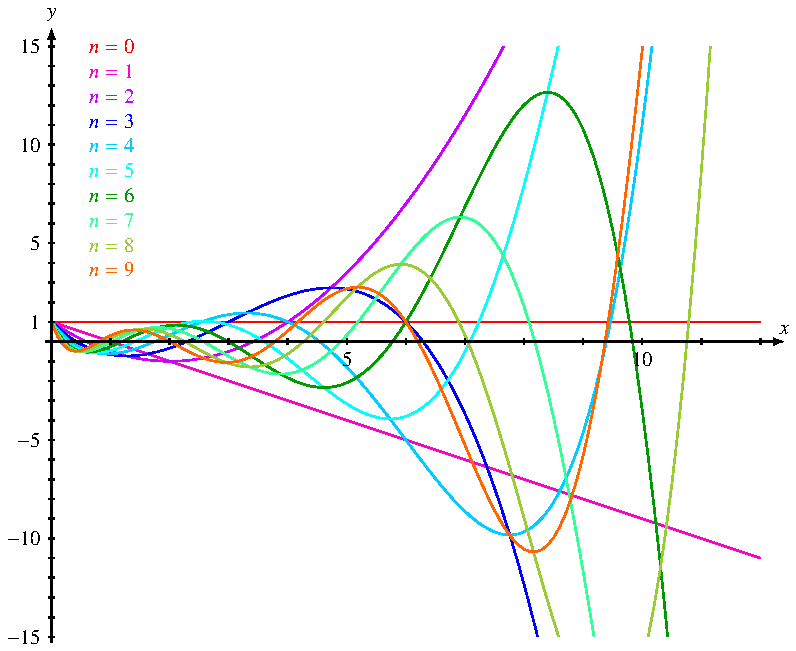
\includegraphics{chapters/070-orthogonalitaet/images/laguerre.pdf}
\caption{Laguerre-Polynome vom Grad $0$ bis $9$
\label{buch:orthogonal:fig:laguerre}}
\end{figure}
\begin{table}
\renewcommand{\arraystretch}{1.4}
\centering
\begin{tabular}{|>{$}c<{$}|>{$}l<{$}|}
\hline
n& L_n(x)\\
\hline
0&1\\
1&-x+1\\
2&\frac1{2!}(x^2-4x+2)\\
3&\frac{1}{3!}(-x^3+9x^2-18x+6)\\
4&\frac{1}{4!}(x^4-16x^3+72x^2-96x+24)\\
5&\frac{1}{5!}(-x^5+25x^4-200x^3+60x^2-600x+120)\\
6&\frac{1}{6!}(x^6-36x^5+450x^4-2400x^3+5400x^2-4320x+720)\\
7&\frac{1}{7!}(-x^7+49x^6-882x^5+7350x^4-29400x^3+52920x^2-35280x+5040)\\
8&\frac{1}{8!}(x^8-64x^7+1568x^6-18816x^5+117600x^4-376320x^3+564480x^2-322560x+40320)\\
\hline
\end{tabular}
\caption{Laguerre-Polynome $L_n(x)$ für $n=0,\dots,8$
\label{buch:orthogonal:table:laguerre}}
\end{table}


